\documentclass[border=10pt]{standalone}

\usepackage{tikz}
\usepackage{tikzsymbols}
\usetikzlibrary{calc,patterns,shapes.geometric}

\def\centerarc[#1](#2)(#3:#4:#5){\draw[#1] ($(#2)+({#5*cos(#3)},{#5*sin(#3)})$) arc (#3:#4:#5);}

\begin{document}
	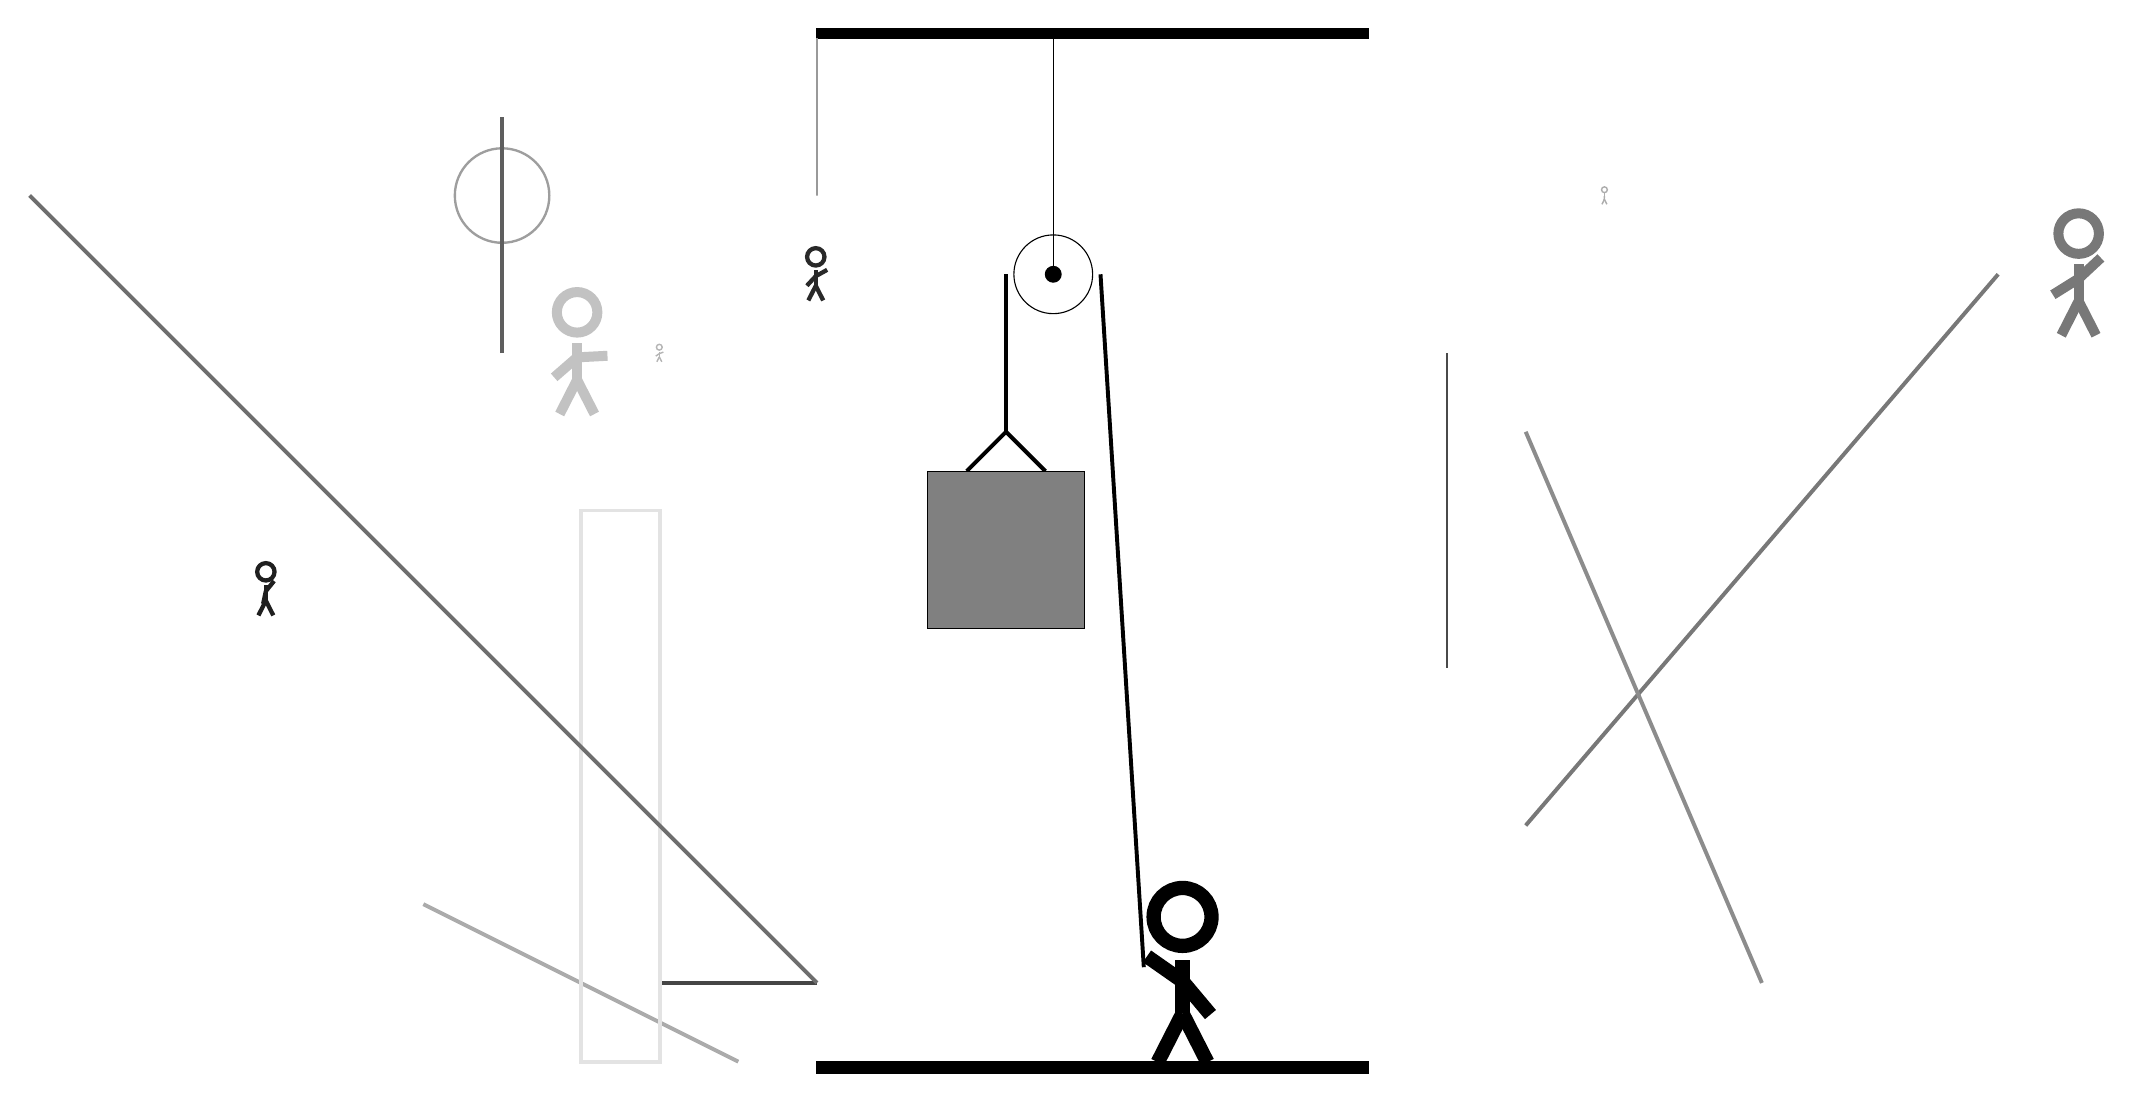
\begin{tikzpicture}
		%%%%% START %%%%%
		
		\draw[fill=black] (-2, 10) rectangle (5, 10.125);
		
		\draw (1, 7) circle (0.5);
		\draw[fill=black] (1, 7) circle (0.1);
		\draw (1, 10) -- (1, 7);
		
		\draw[line width=0.5mm] (-0.1, 4.5) -- (0.4, 5.0) -- (0.9, 4.5);
		\draw[fill=black!50] (-0.6, 4.5) rectangle (1.4, 2.5);
		
		\draw[line width=0.5mm] (0.4, 7) -- (0.4, 5.0);
		\centerarc[line width=0.5mm](1, 7)(0:180:0.6);
		\draw[line width=0.5mm](1.6, 7) -- (2.15, -1.8);
		
		\node at (2.6, -1.9) {\Strichmaxerl[10][-35][-50]};
		
		\draw [line width=0.3mm, color=black!38](-6, 8) circle (0.6);
		
		\draw[line width=0.3mm, color=black!10] (-4, 4) rectangle (-4, 2);
		\draw[line width=0.5mm, color=black!53](7, 0) -- (13, 7);
		\node[line width=0.5mm, color=black!84] at (-2, 7) {\Strichmaxerl[3][47][29]};
		\node[line width=0.6mm, color=black!88] at (-9, 3) {\Strichmaxerl[3][78][51]};
		\node[line width=0.6mm, color=black!53] at (14, 7) {\Strichmaxerl[7][32][43]};
		\draw[line width=0.3mm, color=black!71] (6, 2) rectangle (6, 6);
		\draw[line width=0.3mm, color=black!40] (-2, 10) rectangle (-2, 8);
		\node[line width=0.4mm, color=black!29] at (-4, 6) {\Strichmaxerl[1][35][21]};
		\draw[line width=0.5mm, color=black!45](7, 5) -- (10, -2);
		\draw[line width=0.5mm, color=black!73](-4, -2) -- (-2, -2);
		
		\node[line width=0.2mm, color=black!32] at (8, 8) {\Strichmaxerl[1][86][90]};
		\draw[line width=0.5mm, color=black!33](-3, -3) -- (-7, -1);
		
		\draw[line width=0.5mm, color=black!63](-6, 6) -- (-6, 9);
		\node[line width=0.3mm, color=black!24] at (-5, 6) {\Strichmaxerl[7][41][3]};
		\draw[line width=0.5mm, color=black!11] (-4, -3) rectangle (-5, 4);
		\draw[line width=0.5mm, color=black!57](-2, -2) -- (-12, 8);
		
		
		\draw[fill=black] (-2, -3) rectangle (5, -3.15);
		
		%%%%% END %%%%%
	\end{tikzpicture}
\end{document}